% Options for packages loaded elsewhere
\PassOptionsToPackage{unicode}{hyperref}
\PassOptionsToPackage{hyphens}{url}
%
\documentclass[
  8pt,
  ignorenonframetext,
]{beamer}
\usepackage{pgfpages}
\setbeamertemplate{caption}[numbered]
\setbeamertemplate{caption label separator}{: }
\setbeamercolor{caption name}{fg=normal text.fg}
\beamertemplatenavigationsymbolsempty
% Prevent slide breaks in the middle of a paragraph
\widowpenalties 1 10000
\raggedbottom
\setbeamertemplate{part page}{
  \centering
  \begin{beamercolorbox}[sep=16pt,center]{part title}
    \usebeamerfont{part title}\insertpart\par
  \end{beamercolorbox}
}
\setbeamertemplate{section page}{
  \centering
  \begin{beamercolorbox}[sep=12pt,center]{part title}
    \usebeamerfont{section title}\insertsection\par
  \end{beamercolorbox}
}
\setbeamertemplate{subsection page}{
  \centering
  \begin{beamercolorbox}[sep=8pt,center]{part title}
    \usebeamerfont{subsection title}\insertsubsection\par
  \end{beamercolorbox}
}
\AtBeginPart{
  \frame{\partpage}
}
\AtBeginSection{
  \ifbibliography
  \else
    \frame{\sectionpage}
  \fi
}
\AtBeginSubsection{
  \frame{\subsectionpage}
}
\usepackage{amsmath,amssymb}
\usepackage{lmodern}
\usepackage{iftex}
\ifPDFTeX
  \usepackage[T1]{fontenc}
  \usepackage[utf8]{inputenc}
  \usepackage{textcomp} % provide euro and other symbols
\else % if luatex or xetex
  \usepackage{unicode-math}
  \defaultfontfeatures{Scale=MatchLowercase}
  \defaultfontfeatures[\rmfamily]{Ligatures=TeX,Scale=1}
\fi
% Use upquote if available, for straight quotes in verbatim environments
\IfFileExists{upquote.sty}{\usepackage{upquote}}{}
\IfFileExists{microtype.sty}{% use microtype if available
  \usepackage[]{microtype}
  \UseMicrotypeSet[protrusion]{basicmath} % disable protrusion for tt fonts
}{}
\makeatletter
\@ifundefined{KOMAClassName}{% if non-KOMA class
  \IfFileExists{parskip.sty}{%
    \usepackage{parskip}
  }{% else
    \setlength{\parindent}{0pt}
    \setlength{\parskip}{6pt plus 2pt minus 1pt}}
}{% if KOMA class
  \KOMAoptions{parskip=half}}
\makeatother
\usepackage{xcolor}
\newif\ifbibliography
\setlength{\emergencystretch}{3em} % prevent overfull lines
\providecommand{\tightlist}{%
  \setlength{\itemsep}{0pt}\setlength{\parskip}{0pt}}
\setcounter{secnumdepth}{-\maxdimen} % remove section numbering
% type setting
% ------------------------------------------------------------------------------
\usepackage[german]{babel}     

% fonts
% ------------------------------------------------------------------------------
\usefonttheme{professionalfonts}

% slide title and horizontal line
% ------------------------------------------------------------------------------
\setbeamertemplate{frametitle}{%
    \vskip-30pt \color{black}\large%
    \begin{minipage}[b][23pt]{120mm}%
    \flushleft\insertframetitle%
    \end{minipage}%
}

\setbeamertemplate{headline}										
{
\vskip10pt\hfill\hspace{3.5mm} 										 
\vskip15pt\color{black}\rule{\textwidth}{0.4pt} 					 
}

% slide number
% ---------------------------------------------------------------
\setbeamertemplate{navigation symbols}{}
\setbeamertemplate{footline}
{
\vskip5pt
\vskip2pt
\makebox[123mm]{\hspace{7.5mm}
\hfill Wahrscheinlichkeitstheorie und Frequentistische Inferenz $\vert$ 
\copyright $ $ 2023 Dirk Ostwald CC BY-SA 4.0 $\vert$ 
Folie \insertframenumber}
\vskip4pt
}

% block color scheme
% ------------------------------------------------------------------------------
% colors
\definecolor{white}{RGB}{255,255,255}
\definecolor{grey}{RGB}{235,235,235}
\definecolor{lightgrey}{RGB}{245,245,245}
\definecolor{LightBlue}{RGB}{220,220,255}
\definecolor{darkblue}{RGB}{51, 51, 153}

% definitions and theorems
\setbeamercolor{block title}{fg = black, bg = grey}
\setbeamercolor{block body}{fg = black, bg = lightgrey}

% general line spacing 
% ------------------------------------------------------------------------------
\linespread{1.3}

% local line spacing
% ------------------------------------------------------------------------------
\usepackage{setspace}

% colors
% -----------------------------------------------------------------------------
\usepackage{color}

% justified text
% ------------------------------------------------------------------------------
\usepackage{ragged2e}
\usepackage{etoolbox}
\apptocmd{\frame}{}{\justifying}{}

% bullet point lists
% -----------------------------------------------------------------------------
\setbeamertemplate{itemize item}[circle]
\setbeamertemplate{itemize subitem}[circle]
\setbeamertemplate{itemize subsubitem}[circle]
\setbeamercolor{itemize item}{fg = black}
\setbeamercolor{itemize subitem}{fg = black}
\setbeamercolor{itemize subsubitem}{fg = black}
\setbeamercolor{enumerate item}{fg = black}
\setbeamercolor{enumerate subitem}{fg = black}
\setbeamercolor{enumerate subsubitem}{fg = black}
\setbeamerfont{itemize/enumerate body}{}
\setbeamerfont{itemize/enumerate subbody}{size = \normalsize}
\setbeamerfont{itemize/enumerate subsubbody}{size = \normalsize}

% color links
% ------------------------------------------------------------------------------
\usepackage{hyperref}
\definecolor{urls}{RGB}{204,0,0}
\hypersetup{colorlinks, citecolor = darkblue, urlcolor = urls}


% additional math commands
% ------------------------------------------------------------------------------
\usepackage{bm}                                          
\newcommand{\niton}{\not\owns}
\newcommand{\ups}{\upsilon}

% text highlighting
% ------------------------------------------------------------------------------
\usepackage{soul}
\makeatletter
\let\HL\hl
\renewcommand\hl{%
  \let\set@color\beamerorig@set@color
  \let\reset@color\beamerorig@reset@color
  \HL}
\makeatother

% equation highlighting
% -----------------------------------------------------------------------------
\newcommand{\highlight}[2][yellow]{\mathchoice%
  {\colorbox{#1}{$\displaystyle#2$}}%
  {\colorbox{#1}{$\textstyle#2$}}%
  {\colorbox{#1}{$\scriptstyle#2$}}%
  {\colorbox{#1}{$\scriptscriptstyle#2$}}}%

% additional mathematical operators
% ------------------------------------------------------------------------------
\DeclareMathOperator*{\argmax}{arg\,max}
\DeclareMathOperator*{\argmin}{arg\,min}

\ifLuaTeX
  \usepackage{selnolig}  % disable illegal ligatures
\fi
\IfFileExists{bookmark.sty}{\usepackage{bookmark}}{\usepackage{hyperref}}
\IfFileExists{xurl.sty}{\usepackage{xurl}}{} % add URL line breaks if available
\urlstyle{same} % disable monospaced font for URLs
\hypersetup{
  hidelinks,
  pdfcreator={LaTeX via pandoc}}

\author{}
\date{\vspace{-2.5em}}

\begin{document}

\begin{frame}[plain]{}
\protect\hypertarget{section}{}
\center

\begin{center}
\includegraphics[width=0.2\linewidth]{5_Abbildungen/wtfi_5_otto} \end{center}

\vspace{2mm}

\Large

Wahrscheinlichkeitstheorie und Frequentistische Inferenz \vspace{6mm}

\large

BSc Psychologie WiSe 2022/23

\vspace{6mm}
\large

Prof.~Dr.~Dirk Ostwald
\end{frame}

\begin{frame}[plain]{}
\protect\hypertarget{section-1}{}
\vfill
\center
\huge

\textcolor{black}{(5) Multivariate Verteilungen} \vfill
\end{frame}

\begin{frame}{}
\protect\hypertarget{section-2}{}
\begin{center}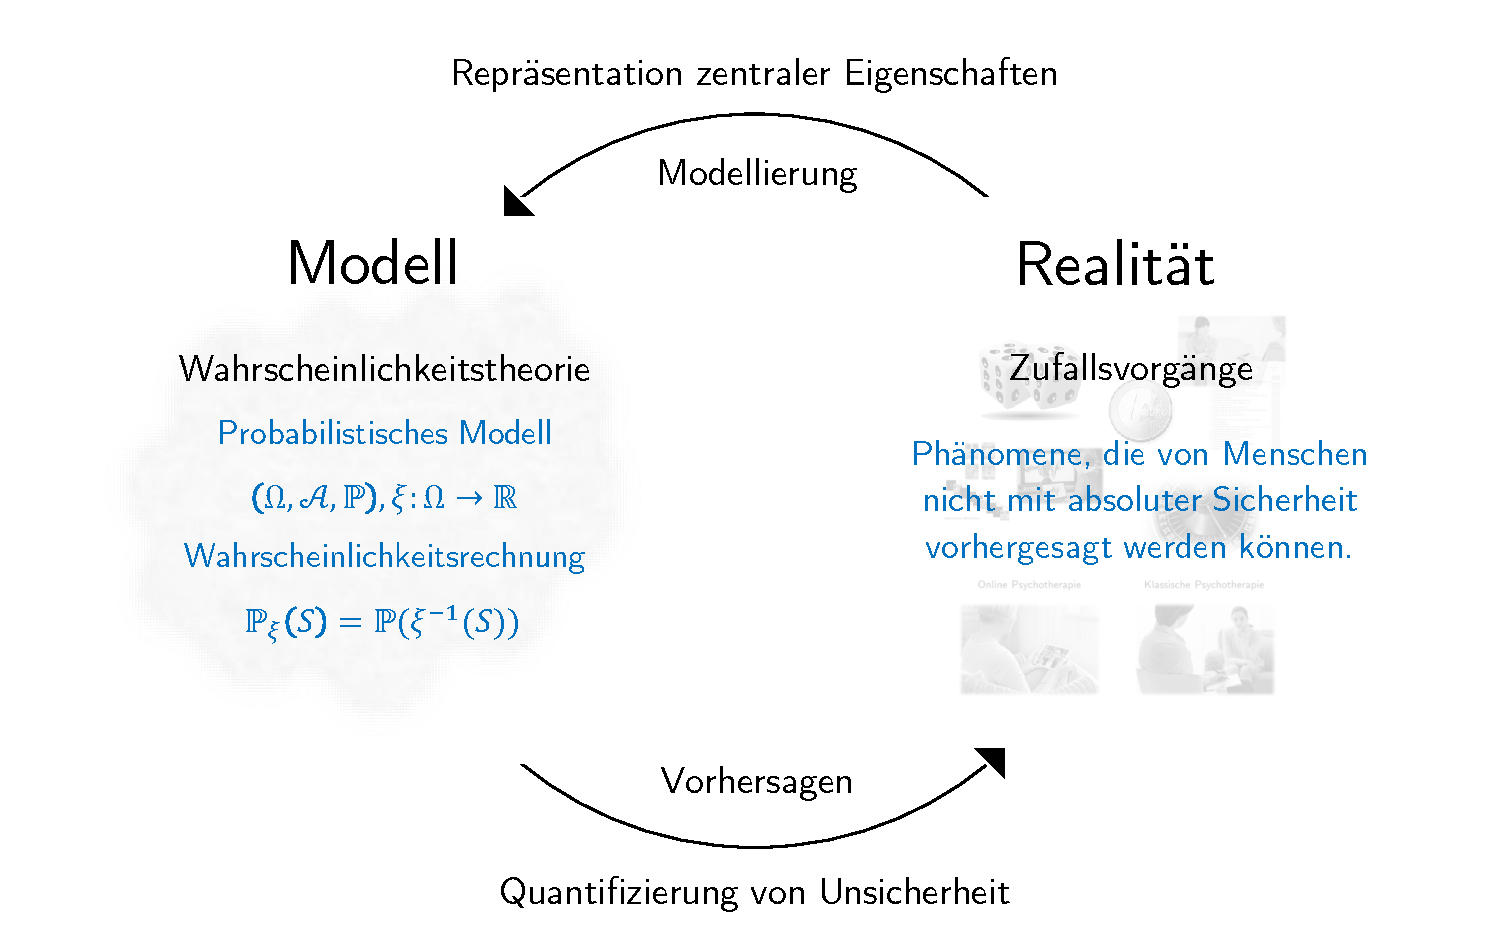
\includegraphics[width=0.95\linewidth]{5_Abbildungen/wtfi_5_wahrscheinlichkeitstheorie_modell} \end{center}
\end{frame}

\begin{frame}{}
\protect\hypertarget{section-3}{}
\vspace{4mm}

\begin{center}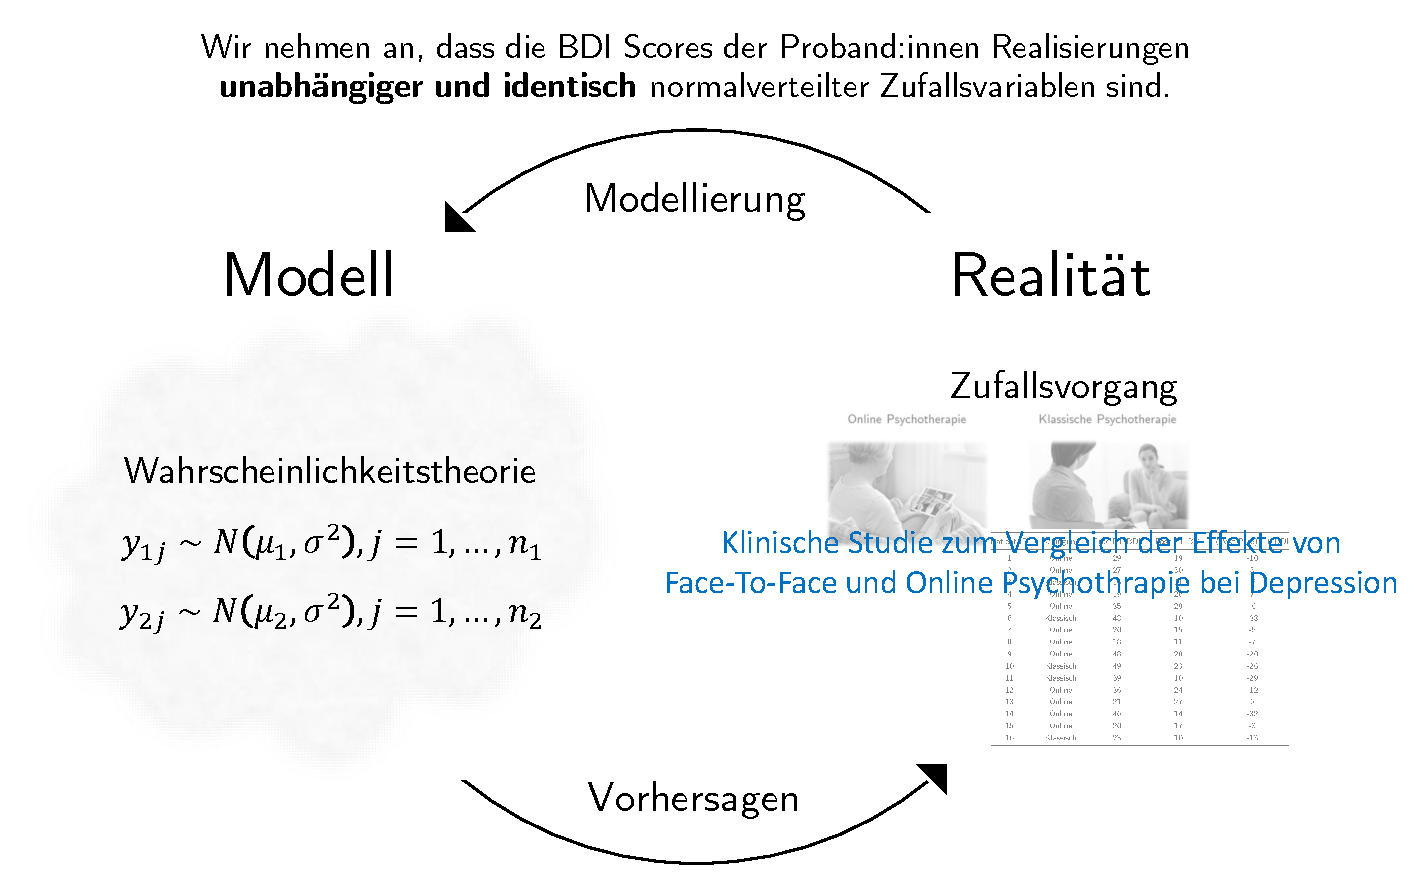
\includegraphics[width=0.9\linewidth]{5_Abbildungen/wtfi_5_wahrscheinlichkeitstheorie_modell_beispiel} \end{center}
\end{frame}

\begin{frame}{}
\protect\hypertarget{section-4}{}
\large
\setstretch{2.2}
\vfill

Definition

Multivariate Verteilungen

Marginalverteilungen

Bedingte Verteilungen

Unabhängige Zufallsvariablen

Selbstkontrollfragen

\vfill
\end{frame}

\begin{frame}{}
\protect\hypertarget{section-5}{}
\large
\setstretch{2.2}
\vfill

\textbf{Definition}

Multivariate Verteilungen

Marginalverteilungen

Bedingte Verteilungen

Unabhängige Zufallsvariablen

Selbstkontrollfragen

\vfill
\end{frame}

\begin{frame}{Definition}
\protect\hypertarget{definition}{}
\small
\begin{definition}[Zufallsvektor]
\justifying
$(\Omega, \mathcal{A}, \mathbb{P})$ sei ein Wahrscheinlichkeitsraum und 
$(\mathcal{X},\mathcal{S})$ sei ein $n$-dimensionaler Messraum. 
Ein $n$-dimensionaler \textit{Zufallsvektor} ist definiert als eine Abbildung
\begin{equation}
\xi:\Omega \to \mathcal{X}, \omega \mapsto \xi(\omega) :=
\begin{pmatrix}
\xi_1(\omega) \\
\vdots      \\
\xi_n(\omega)
\end{pmatrix}
\end{equation}
mit der \textit{Messbarkeitseigenschaft}
\begin{equation}
\{\omega \in \Omega|\xi(\omega) \in S \} \in \mathcal{A} \mbox{ für alle } S \in \mathcal{S}.
\end{equation}
\end{definition}
\vspace{-2mm}
\footnotesize

Bemerkungen \vspace{-2mm}

\begin{itemize}
\tightlist
\item
  \(\xi\) ist hier eine univariate, vektorwertige Abbildung.
\item
  Das Standardbeispiel für \((\mathcal{X},\mathcal{S})\) ist
  \((\mathbb{R}^n, \mathcal{B}(\mathbb{R}^n))\).
\item
  Wir verzichten auf eine explizite Einführung \(n\)-dimensionaler
  \(\sigma\)-Algebren wie \(\mathcal{B}(\mathbb{R}^n)\).
\item
  Ohne Beweis halten wir fest, dass \(\xi\) messbar ist, wenn die
  Funktionen \(\xi_1,...,\xi_n\) messbar sind.
\item
  Die Komponentenfunktionen eines Zufallsvektors sind Zufallsvariablen.
\item
  Ein \(n\)-dimensionaler Zufallsvektor ist die Konkatenation von \(n\)
  Zufallsvariablen.
\item
  Für \(n := 1\) ist ein Zufallsvektor eine Zufallsvariable.
\item
  Für einen Zufallsvektor schreiben wir auch häufig
  \(\xi:= (\xi_1,...,\xi_n)\).
\end{itemize}
\end{frame}

\begin{frame}{Definition}
\protect\hypertarget{definition-1}{}
\vspace{.2cm}
\center

\begin{center}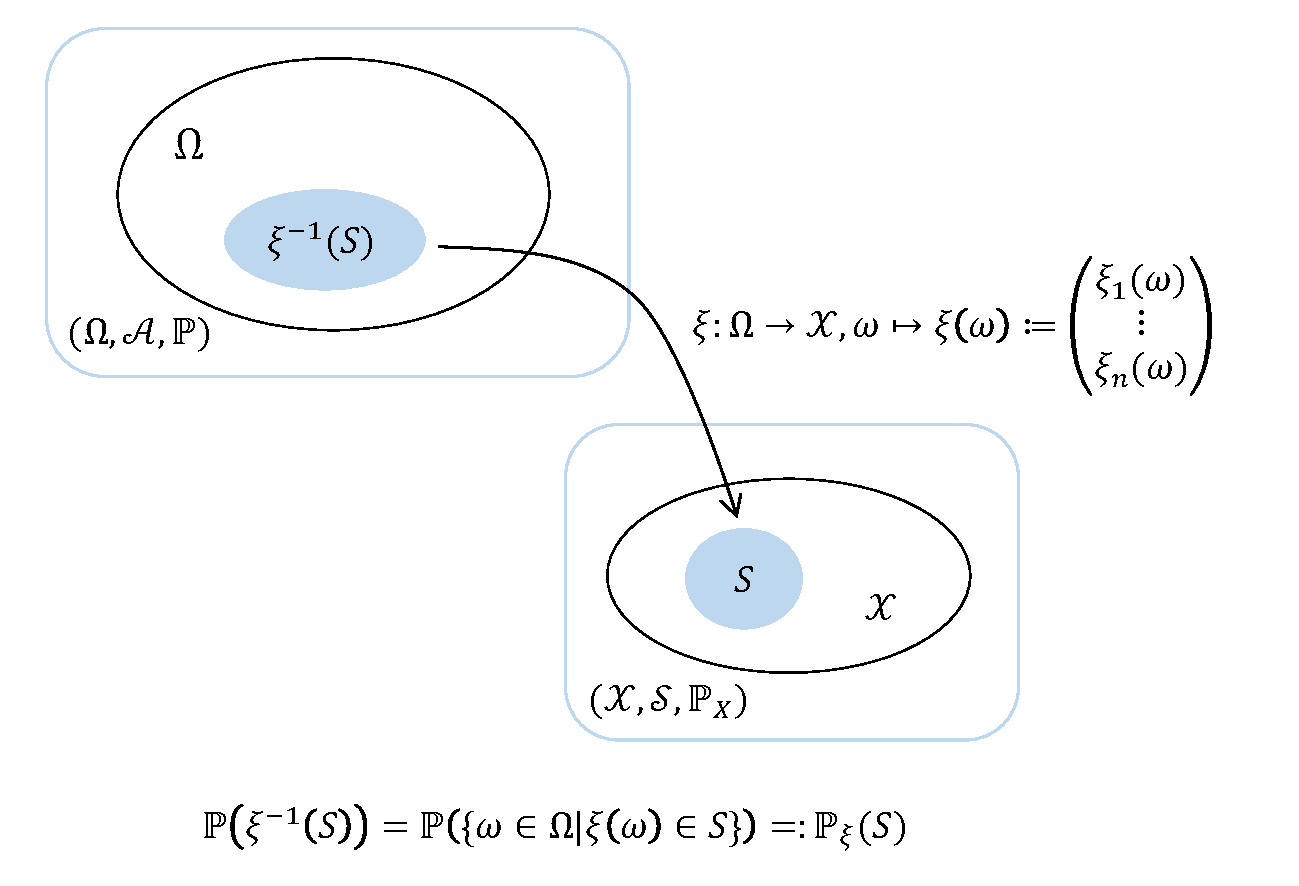
\includegraphics[width=1\linewidth]{5_Abbildungen/wtfi_5_zufallsvektor} \end{center}
\end{frame}

\begin{frame}{}
\protect\hypertarget{section-6}{}
\large
\setstretch{2.2}
\vfill

Definition

\textbf{Multivariate Verteilungen}

Marginalverteilungen

Bedingte Verteilungen

Unabhängige Zufallsvariablen

Selbstkontrollfragen

\vfill
\end{frame}

\begin{frame}{Multivariate Verteilungen}
\protect\hypertarget{multivariate-verteilungen}{}
\small
\begin{definition}[Multivariate Verteilung]
\justifying
$(\Omega, \mathcal{A}, \mathbb{P})$ sei ein Wahrscheinlichkeitsraum, 
$(\mathcal{X},\mathcal{S})$ sei ein $n$-dimensionaler Messraum und
\begin{equation}
\xi : \Omega \to \mathcal{X}, \omega \mapsto \xi(\omega)
\end{equation}
sei ein Zufallsvektor. Dann heißt das Wahrscheinlichkeitsmaß $\mathbb{P}_\xi$, 
definiert durch
\begin{equation}
\mathbb{P}_\xi : \mathcal{S} \to [0,1], S \mapsto \mathbb{P}_\xi(S)
:= \mathbb{P}(\xi^{-1}(S))
 = \mathbb{P}\left(\{\omega \in \Omega|\xi(\omega) \in S\}\right)
\end{equation}
die \textit{multivariate Verteilung des Zufallsvektor $\xi$}.
\end{definition}
\footnotesize

Bemerkungen

\begin{itemize}
\tightlist
\item
  Der Einfachheit halber spricht man oft auch nur von ``der Verteilung
  des Zufallsvektors \(\xi\)''.
\item
  Die Notationskonventionen für Zufallsvariablen gelten für
  Zufallsvektoren analog, z.B. \begin{align}
  \begin{split}
  \mathbb{P}_\xi(\xi \in S)
  & := \mathbb{P}\left(\{\xi \in S\} \right)
  = \mathbb{P}\left(\{\omega \in \Omega|\xi(\omega) \in S\} \right)
  \\
  \mathbb{P}_\xi(\xi = x)
  & := \mathbb{P}\left(\{\xi = x\} \right)
  = \mathbb{P}\left(\{\omega \in \Omega|\xi(\omega) = x\} \right)
  \\
  \mathbb{P}_\xi(\xi \le x)
  & := \mathbb{P}\left(\{\xi \le x\} \right)
  = \mathbb{P}\left(\{\omega \in \Omega|\xi(\omega) \le x\} \right)
  \\
  \mathbb{P}_\xi(x_1 \le \xi \le x_2)
  & := \mathbb{P}\left(\{x_1 \le \xi \le x_2\} \right)
   = \mathbb{P}\left(\{\omega \in \Omega|x_1 \le \xi(\omega) \le x_2\} \right)
  \end{split}
  \end{align}
\item
  Relationsoperatoren wie \(\le\) werden hier \textit{komponentenweise}
  verstanden.
\item
  Zum Beispiel heißt \(x \le y\) für \(x,y \in \mathbb{R}^n\), dass
  \(x_i \le y_i\) für alle \(i = 1,...,n\).
\end{itemize}
\end{frame}

\begin{frame}{Multivariate Verteilungen}
\protect\hypertarget{multivariate-verteilungen-1}{}
\small
\begin{definition}[Multivariate kumulative Verteilungsfunktionen]
$\xi$ sei ein Zufallsvektor mit Ergebnisraum $\mathcal{X}$. Dann heißt eine Funktion
der Form
\begin{equation}
P_\xi : \mathcal{X} \to [0,1],\, x \mapsto P_\xi(x) := \mathbb{P}_\xi(\xi \le x)
\end{equation}
multivariate kumulative Verteilungsfunktion von $\xi$.
\end{definition}

Bemerkung

\begin{itemize}
\tightlist
\item
  \justifying Multivariate kumulative Verteilungsfunktionen können zur
  Definition von multivariaten Verteilungen genutzt werden, häufiger ist
  allerdings die Definition multivariater Verteilungen durch
  multivariate Wahrscheinlichkeitsmasse- oder
  Wahrscheinlichkeitsdichtefunktionen.
\end{itemize}
\end{frame}

\begin{frame}{Multivariate Verteilungen}
\protect\hypertarget{multivariate-verteilungen-2}{}
\small
\begin{definition}[Diskreter Zufallsvektor, Multivariate WMF]
\justifying
$\xi$ sei ein Zufallsvektor mit Ergebnisraum $\mathcal{X}$. $\xi$ heißt 
\textit{diskreter Zufallsvektor} wenn der Ergebnisraum $\mathcal{X}$ endlich oder
abzählbar ist und eine Funktion 
\begin{equation}
p_\xi : \mathcal{X} \to [0,1], x \mapsto p_\xi(x)  
\end{equation}
existiert, für die gilt
\begin{itemize}
\item[(1)] $\sum_{x \in \mathcal{X}}p(x) = 1$ und
\item[(2)] $\mathbb{P}_\xi(\xi = x) = p(x)$ für alle $x \in \mathcal{X}$.
\end{itemize}
Ein entsprechende Funktion $p$ heißt \textit{multivariate Wahrscheinlichkeitsmassefunktion (WMF)} von $\xi$.
\end{definition}

Bemerkungen

\begin{itemize}
\tightlist
\item
  Der Begriff der multivariaten WMF ist analog zum Begriff der WMF.
\item
  Man spricht oft einfach von der WMF eines Zufallsvektors.
\item
  Wie univariate WMFen sind multivariate WMFen nicht-negativ und
  normiert.
\end{itemize}
\end{frame}

\begin{frame}{Multivariate Verteilungen}
\protect\hypertarget{multivariate-verteilungen-3}{}
Beispiel (Multivariate Wahrscheinlichkeitsmassefunktion)

\vspace{2mm}

\small
\justifying

Wir betrachten einen zweidimensionalen Zufallsvektor
\(\xi:= (\xi_1,\xi_2)\) der Werte in
\(\mathcal{X} := \mathcal{X}_1 \times \mathcal{X}_2\) annimmt, wobei
\(\mathcal{X}_1 := \{1,2,3\}\) und \(\mathcal{X}_2 = \{1,2,3,4\}\)
seien.

Eine exemplarische bivariate WMF der Form \begin{equation}
p_\xi: \{1,2,3\} \times \{1,2,3,4\} \to [0,1], (x_1,x_2) \mapsto p_\xi(x_1,x_2)
\end{equation} ist dann durch nachfolgende Tabelle definiert:
\vspace{1mm}

\begin{table}\label{tab:wmf_bivariat}
\begin{center}
\begin{tabular}{|c|cccc|}
\hline
$p_\xi(x_1,x_2)$    &   $x_2 = 1$   &   $x_2 = 2$   &   $x_2 = 3$   &   $x_2 = 4$   \\\hline
$x_1 = 1$       &   $0.1$       &   $0.0$       &   $0.2$       &   $0.1$       \\
$x_1 = 2$       &   $0.1$       &   $0.2$       &   $0.0$       &   $0.0$       \\
$x_1 = 3$       &   $0.0$       &   $0.1$       &   $0.1$       &   $0.1$       \\\hline
\end{tabular}
\end{center}
\end{table}
\vspace{1mm}

Man beachte, dass
\(\sum_{x_1 = 1}^3 \sum_{x_2 = 1}^4 p_\xi(x_1,x_2) = 1\).
\end{frame}

\begin{frame}{Multivariate Verteilungen}
\protect\hypertarget{multivariate-verteilungen-4}{}
\small
\begin{definition}[Kontinuierlicher Zufallsvektor, Multivariate WDF]
\justifying
Ein Zufallsvektor $\xi$ heißt \textit{kontinuierlich}, wenn $\mathbb{R}^n$ der 
Ergebnisraum von $\xi$ ist und eine Funktion  
\begin{equation}
p_\xi : \mathbb{R}^n \to \mathbb{R}_{\ge 0}, x \mapsto p_\xi(x),
\end{equation}
existiert, für die gilt
\begin{itemize}
\item[(1)] $\int_{\mathbb{R}^n} p_\xi(x)\,dx = 1$ und
\item[(2)] $\mathbb{P}_\xi(x_1 \le \xi \le x_2)
            = \int_{x_{1_1}}^{x_{2_1}} \cdots \int_{x_{1_n}}^{x_{2_n}} p_\xi(s_1,...,s_n)\,ds_1 \cdots ds_n$.
\end{itemize}
Eine entsprechende Funktion $p$ heißt \textit{multivariate Wahrscheinlichkeitsdichtefunktion (WDF)} von $\xi$.
\end{definition}

Bemerkungen

\begin{itemize}
\tightlist
\item
  Der Begriff der multivariaten WDF ist analog zum Begriff der WDF.
\item
  Man spricht häufig auch einfach von der WDF eines Zufallsvektors
\item
  Wie univariate WDFen sind multivariate WDFen nicht-negativ und
  normiert.
\item
  Wie für kontinuierliche Zufallsvariablen gilt für kontinuierliche
  Zufallsvektoren \begin{equation}
  \mathbb{P}_\xi(\xi = x)
  = \mathbb{P}_\xi(x \le \xi \le x)
  = \int_{x_1}^{x_1} \cdots \int_{x_n}^{x_n} p_\xi(s_1,...,s_n)\,ds_1 \cdots ds_n
  = 0
  \end{equation}
\end{itemize}
\end{frame}

\begin{frame}{}
\protect\hypertarget{section-7}{}
\large
\setstretch{2.2}
\vfill

Definition

Multivariate Verteilungen

\textbf{Marginalverteilungen}

Bedingte Verteilungen

Unabhängige Zufallsvariablen

Selbstkontrollfragen

\vfill
\end{frame}

\begin{frame}{Marginalverteilungen}
\protect\hypertarget{marginalverteilungen}{}
\small
\begin{definition}[Univariate Marginalverteilung]
\justifying
$(\Omega, \mathcal{A}, \mathbb{P})$ sei ein Wahrscheinlichkeitsraum, 
$(\mathcal{X}, \mathcal{S})$ sei ein $n$-dimensionaler Messraum, 
$\xi:\Omega \to \mathcal{X}$ sei ein Zufallsvektor, $\mathbb{P}_\xi$ sei die 
Verteilung von $\xi$, $\mathcal{X}_i \subset \mathcal{X}$ sei der Ergebnisraum der 
$i$ten Komponente $\xi_i$ von $\xi$, und $\mathcal{S}_i$ sei eine 
$\sigma$-Algebra auf $\xi_i$. Dann heißt die durch
\begin{equation}
\mathbb{P}_{\xi_i} : \mathcal{S}_i \to [0,1],
S \mapsto  \mathbb{P}_\xi\left(\mathcal{X}_1
                     \times
                     \cdots
                     \times
                     \mathcal{X}_{i-1}
                     \times S
                     \times \mathcal{X}_{i+1}
                     \times \cdots
                     \times \mathcal{X}_n\right)
\mbox{ für } S \in \mathcal{S}_i
\end{equation}
definierte Verteilung die \textit{$i$te univariate Marginalverteilung von $\xi$}.
\end{definition}

Bemerkungen

\begin{itemize}
\tightlist
\item
  \justifying Univariate Marginalverteilungen sind die Verteilungen der
  Komponenten eines Zufallsvektors.
\item
  Univariate Marginalverteilungen sind Verteilungen von
  Zufallsvariablen.
\item
  Die Festlegung der multivariaten Verteilung von \(\xi\) legt auch die
  Verteilungen der \(\xi_i\) fest.
\end{itemize}
\end{frame}

\begin{frame}{Marginalverteilungen}
\protect\hypertarget{marginalverteilungen-1}{}
\footnotesize
\begin{theorem}[Marginale Wahrscheinlichkeitsmasse- und dichtefunktionen]
\justifying
\normalfont
(1) $\xi= (\xi_1,...,\xi_n)$ sei ein $n$-dimensionaler diskreter Zufallsvektor
mit Wahrscheinlichkeitsmassefunktion $p_\xi$ und Komponentenergebnisräumen 
$\mathcal{X}_1, ..., \mathcal{X}_n$. Dann ergibt sich die 
Wahrscheinlichkeitsmassefunktion der $i$ten Komponente $\xi_i$ von $\xi$ als
\begin{multline}
p_{\xi_i} : \mathcal{X}_i \to [0,1], x_i \mapsto p_{\xi_i}(x_i) := \\
\sum_{x_1} \cdots \sum_{x_{i-1}} \sum_{x_{i+1}} \cdots \sum_{x_n} p_\xi(x_1,...,x_{i-1},x_i,x_{i+1}, ...,x_n).
\end{multline}
(2) $\xi= (\xi_1,...,\xi_n)$ sei ein $n$-dimensionaler kontinuierlicher Zufallsvektor 
mit Wahrscheinlichkeitsdichtefunktion $p_\xi$ und Komponentenergebnisraum $\mathbb{R}$. 
Dann ergibt sich die Wahrscheinlichkeitsdichtefunktion der $i$ten Komponente $\xi_i$ von $\xi$ als
\begin{multline}
p_{\xi_i} : \mathbb{R} \to \mathbb{R}_{\ge 0},  x_i \mapsto p_{\xi_i}(x_i) :=  \\
\smallint_{x_1} \cdots \smallint_{x_{i-1}} \smallint_{x_{i+1}} \cdots \smallint_{x_n}
   p_\xi(x_1,..., x_{i-1},x_i,x_{i+1}, ...,x_n)
   \,dx_1...\,dx_{i-1}\,dx_{i+1}...\,dx_n.
\end{multline}
\end{theorem}
\vspace{-2mm}

Bemerkungen \vspace{-1mm}

\begin{itemize}
\tightlist
\item
  \justifying Wir verzichten auf einen Beweis.
\item
  Die WMFen der univariaten Marginalverteilungen diskreter
  Zufallsvektoren ergeben sich durch Summation.
\item
  Die WDFen der univariaten Marginalverteilungen kontinuierlicher
  Zufallsvektoren ergeben sich durch Integration.
\end{itemize}
\end{frame}

\begin{frame}{Marginalverteilungen}
\protect\hypertarget{marginalverteilungen-2}{}
Beispiel (Marginale Wahrscheinlichkeitsmassefunktionen)

\vspace{2mm}

\small
\justifying

Wir betrachten erneut den zweidimensionalen Zufallsvektor
\(\xi:= (\xi_1,\xi_2)\) der Werte in
\(\mathcal{X} := \mathcal{X}_1 \times \mathcal{X}_2\) annimmt, wobei
\(\mathcal{X}_1 := \{1,2,3\}\) und \(\mathcal{X}_2 = \{1,2,3,4\}\)
seien. \vspace{1mm}

Basierend auf der oben definierten WMF ergeben sich folgende marginale
WMFen \(p_{\xi_1}\) und \(p_{\xi_2}\): \vspace{2mm}

\begin{table}\label{tab:wmf_marginal}
\begin{center}
\begin{tabular}{|c|cccc|c|}
\hline
$p_\xi(x_1,x_2)$    &   $x_2 = 1$   &   $x_2 = 2$   &   $x_2 = 3$   &   $x_2 = 4$   & $p_{\xi_1}(x_1)$  \\\hline
$x_1 = 1$           &   $0.1$       &   $0.0$       &   $0.2$       &   $0.1$       & $0.4$             \\
$x_1 = 2$           &   $0.1$       &   $0.2$       &   $0.0$       &   $0.0$       & $0.3$             \\
$x_1 = 3$           &   $0.0$       &   $0.1$       &   $0.1$       &   $0.1$       & $0.3$             \\\hline
$p_{\xi_2}(x_2)$    &   $0.2$       &   $0.3$       &   $0.3$       &   $0.2$       &                   \\\hline
\end{tabular}
\end{center}
\end{table}
\vspace{2mm}

Man beachte, dass \(\sum_{x_1 = 1}^3 p_{\xi_1}(x_1) = 1\) und
\(\sum_{x_2 = 1}^3 p_{\xi_2}(x_2) = 1\) gilt.
\end{frame}

\begin{frame}{}
\protect\hypertarget{section-8}{}
\large
\setstretch{2.2}
\vfill

Definition

Multivariate Verteilungen

Marginalverteilungen

\textbf{Bedingte Verteilungen}

Unabhängige Zufallsvariablen

Selbstkontrollfragen

\vfill
\end{frame}

\begin{frame}{Bedingte Verteilungen}
\protect\hypertarget{bedingte-verteilungen}{}
\small

Vorbemerkungen

\footnotesize

Wir erinnern uns, dass für einen Wahrscheinlichkeitsraum
\((\Omega, \mathcal{A}, \mathbb{P})\) und zwei Ereignisse
\(A,B \in \mathcal{A}\) mit \(\mathbb{P}(B) > 0\) die bedingte
Wahrscheinlichkeit von \(A\) gegeben \(B\) definiert ist als
\begin{equation}
\mathbb{P}(A|B) = \frac{\mathbb{P}(A \cap B)}{\mathbb{P}(B)}.
\end{equation}

Analog wird für zwei Zufallsvariablen \(\xi_1,\xi_2\) mit Ereignisräumen
\(\mathcal{X}_1,\mathcal{X}_2\) und (messbaren) Mengen
\(S_1 \in \mathcal{X}_1, S_2 \in \mathcal{X}_2\) die bedingte Verteilung
von \(\xi_1\) gegeben \(\xi_2\) mithilfe der Ereignisse \begin{equation}
A := \{\xi_1 \in S_1\} \mbox{ und } B := \{\xi_2 \in S_2\}
\end{equation} definiert. \vspace{1mm}

So ergibt sich zum Beispiel die bedingte Wahrscheinlichkeit, dass
\(\xi_1 \in S_1\) gegeben dass \(\xi_2 \in S_2\) unter der Annahme, dass
\(\mathbb{P}(\{\xi_2 \in S_2\}) > 0\), zu \begin{equation}
\mathbb{P}( \{\xi_1 \in S_1\}|\{\xi_2 \in S_2\})
= \frac{\mathbb{P}(\{\xi_1 \in S_1\} \cap \{\xi_2 \in S_2\})}{\mathbb{P}(\{\xi_2 \in S_2\})}.
\end{equation}

Wir betrachten zunächst durch WMFen/WDFen zweidimensionaler
Zufallsvektoren definierte bedingte Verteilungen.
\end{frame}

\begin{frame}{Bedingte Verteilungen}
\protect\hypertarget{bedingte-verteilungen-1}{}
\footnotesize
\begin{definition}[Bedingte WMF, diskrete bedingte Verteilung]
\justifying
$\xi:= (\xi_1,\xi_2)$ sei ein diskreter Zufallsvektor mit Ergebnisraum 
$\mathcal{X} := \mathcal{X}_1 \times \mathcal{X}_2$, WMF $p_\xi = p_{\xi_1,\xi_2}$ 
und marginalen WMFen $p_{\xi_1}$ und $p_{\xi_2}$. Die bedingte WMF von $\xi_1$ gegeben 
$\xi_2 = x_2$ ist dann für $p_{\xi_2}(x_2) > 0$ definiert als
\begin{equation}
p_{\xi_1|\xi_2 = x_2} : \mathcal{X}_1 \to [0,1],
x_1 \mapsto p_{\xi_1|\xi_2 = x_2}(x_1|x_2) := \frac{p_{\xi_1,\xi_2}(x_1,x_2)}{p_{\xi_2}(x_2)}
\end{equation}
Analog ist für $p_{\xi_1}(x_1) > 0$ die bedingte WMF von $\xi_2$ gegeben $\xi_1 = x_1$ 
definiert als
\begin{equation}
p_{\xi_2|\xi_1 = x_1} : \mathcal{X}_2 \to [0,1],
x_2 \mapsto p_{\xi_2|\xi_1 = x_2}(x_1|x_2) := \frac{p_{\xi_1,\xi_2}(x_1,x_2)}{p_{\xi_1}(x_1)}
\end{equation}
Die bedingten Verteilungen mit WMFen $p_{\xi_1|\xi_2 = x_2}$ und $p_{\xi_2|\xi_1 = x_1}$ 
heißen dann die \textit{diskreten bedingten Verteilungen von $\xi_1$ gegeben $\xi_2 = x_2$ 
und $\xi_2$ gegeben $\xi_1 = x_1$}, respektive.
\end{definition}

Bemerkungen

\begin{itemize}
\tightlist
\item
  In Analogie zur Definition der bedingten Wahrscheinlichkeit von
  Ereignissen gilt also \begin{equation}
  p_{\xi_1|\xi_2}(x_1|x_2)
  = \frac{p_{\xi_1,\xi_2}(x_1,x_2)}{p_{\xi_2}(x_2)}
  = \frac{\mathbb{P}(\{\xi_1 = x_1\} \cap \{\xi_2 = x_2\})}{\mathbb{P}(\{\xi_2 = x_2\})}.
  \end{equation}
\item
  Bedingte Verteilungen sind (lediglich) normalisierte gemeinsame
  Verteilungen.
\end{itemize}
\end{frame}

\begin{frame}{Bedingte Verteilungen}
\protect\hypertarget{bedingte-verteilungen-2}{}
Beispiel (Bedingte Wahrscheinlichkeitsmassefunktionen)

\vspace{2mm}

\small
\justifying

Wir betrachten erneut den zweidimensionalen Zufallsvektor
\(\xi:= (\xi_1,\xi_2)\) der Werte in
\(\mathcal{X} := \mathcal{X}_1 \times \mathcal{X}_2\) annimmt, wobei
\(\mathcal{X}_1 := \{1,2,3\}\) und \(\mathcal{X}_2 = \{1,2,3,4\}\)
seien.

Basierend auf der oben definierten WMF und den entsprechenden oben
evaluierten marginalen WMFen ergeben sich folgende bedingte WMFen für
\(p_{\xi_2|\xi_1 = x_1}\) \vspace{1mm}

\renewcommand{\arraystretch}{1.4}
\begin{center}
\begin{tabular}{|c|cccc|}
\hline
$p_{\xi_2|\xi_1}(x_2|x_1)$
&   $x_2 = 1$
&   $x_2 = 2$
&   $x_2 = 3$
&   $x_2 = 4$
\\\hline
$p_{\xi_2|\xi_1 = 1}(x_2|x_1 = 1)$

&   $\frac{0.1}{0.4} = 0.25$

&   $\frac{0.0}{0.4} = 0.00$

&   $\frac{0.2}{0.4} = 0.50$

&   $\frac{0.1}{0.4} = 0.25$
\\
$p_{\xi_2|\xi_1 = 2}(x_2|x_1 = 2)$

&   $\frac{0.1}{0.3} = 0.3\bar{3}$

&   $\frac{0.2}{0.3} = 0.6\bar{6}$

&   $\frac{0.0}{0.3} = 0.00$

&   $\frac{0.0}{0.3} = 0.00$
\\
$p_{\xi_2|\xi_1 = 3}(x_2|x_1 = 3)$

&   $\frac{0.0}{0.3} = 0.00$

&   $\frac{0.1}{0.3} = 0.3\bar{3}$

&   $\frac{0.1}{0.3} = 0.3\bar{3}$

&   $\frac{0.1}{0.3} = 0.3\bar{3}$
\\\hline
\end{tabular}
\end{center}

\footnotesize

Bemerkungen

\begin{itemize}
\tightlist
\item
  Man beachte, dass
  \(\sum_{x_2 = 1}^4 p_{\xi_2|\xi_1 = x_1}(x_2|x_1) = 1\) für alle
  \(x_1 \in \mathcal{X}_1\).
\item
  Man beachte die qualitative Ähnlichkeit der WMFen
  \(p_{\xi_1,\xi_2}(x_1,x_2)\) und \(p_{\xi_2|\xi_1}(x_2|x_1)\).
\item
  Bedingte Verteilungen sind (lediglich) normalisierte gemeinsame
  Verteilungen.
\end{itemize}
\end{frame}

\begin{frame}{Bedingte Verteilungen}
\protect\hypertarget{bedingte-verteilungen-3}{}
\footnotesize
\begin{definition}[Bedingte WDF, kontinuierliche bedingte Verteilungen]
\justifying
$\xi:= (\xi_1,\xi_2)$ sei ein kontinuierlicher Zufallsvektor mit Ergebnisraum 
$\mathbb{R}^2$, WDF $p_\xi = p_{\xi_1,\xi_2}$ und marginalen WDFen $p_{\xi_1}$ und $p_{\xi_2}$.
Die bedingte WDF von $\xi_1$ gegeben $\xi_2 = x_2$ ist dann für $p_{\xi_2}(x_2) > 0$ definiert als
\begin{equation}
p_{\xi_1|\xi_2 = x_2} : \mathbb{R} \to \mathbb{R}_{\ge 0},
x_1 \mapsto p_{\xi_1|\xi_2 = x_2}(x_1|x_2) := \frac{p_{\xi_1,\xi_2}(x_1,x_2)}{p_{\xi_2}(x_2)}
\end{equation}
Analog ist für $p_{\xi_1}(x_1) > 0$ die bedingte WMF von $\xi_2$ gegeben $\xi_1 = x_1$ definiert als
\begin{equation}
p_{\xi_2|\xi_1 = x_1} : \mathbb{R} \to \mathbb{R}_{\ge 0},
x_2 \mapsto p_{\xi_2|\xi_1 = x_2}(x_2|x_1) := \frac{p_{\xi_1,\xi_2}(x_1,x_2)}{p_{\xi_1}(x_1)}
\end{equation}

Die Verteilungen mit WDFen $p_{\xi_1|\xi_2 = x_2}$ und $p_{\xi_2|\xi_1 = x_1}$ heißen dann
die \textit{kontinuierlichen bedingten Verteilungen von $\xi_1$ gegeben $\xi_2 = x_2$ 
und $\xi_2$ gegeben $\xi_1 = x_1$}, respektive.
\end{definition}

Bemerkung

\begin{itemize}
\tightlist
\item
  Im kontinuierlichen Fall gilt zwar \(\mathbb{P}(\xi = x) = 0\), aber
  nicht notwendig auch \(p_\xi(x) = 0\).
\end{itemize}
\end{frame}

\begin{frame}{}
\protect\hypertarget{section-9}{}
\large
\setstretch{2.2}
\vfill

Definition

Multivariate Verteilungen

Marginalverteilungen

Bedingte Verteilungen

\textbf{Unabhängige Zufallsvariablen}

Selbstkontrollfragen

\vfill
\end{frame}

\begin{frame}{Unabhängige Zufallsvariablen}
\protect\hypertarget{unabhuxe4ngige-zufallsvariablen}{}
\small
\begin{definition}[Unabhängige Zufallsvariablen]
\justifying
$(\Omega, \mathcal{A}, \mathbb{P})$ sei ein Wahrscheinlichkeitsraum und 
$\xi: = (\xi_1,\xi_2)$ ein zweidimensionaler Zufallsvektor. Die Zufallsvariablen 
$\xi_1,\xi_2$ mit Ergebnisräumen $\mathcal{X}_1, \mathcal{X}_2$ 
heißen \textit{unabhängig}, wenn für alle $S_1 \subseteq \mathcal{X}_1$ und 
$S_2 \subseteq \mathcal{X}_2$ gilt, dass
\begin{equation}
\mathbb{P}_\xi(\xi_1 \in S_1, \xi_2 \in S_2) =
\mathbb{P}_{\xi_1}(\xi_1 \in S_1)\mathbb{P}_{\xi_2}(\xi_2 \in S_2).
\end{equation}
\end{definition}

Bemerkungen

\begin{itemize}
\tightlist
\item
  Die Definition besagt, dass die Ereignisse \(\{\xi_1 \in S_1\}\) und
  \(\{\xi_2 \in S_2\}\) unabhängig sind.
\item
  Es gilt also auch, dass
  \(\mathbb{P}(\{\xi_1 \in S_1\})|\{\xi_2 \in S_2\}) = \mathbb{P}(\{\xi_1 \in S_1\})\).
\item
  Wissen um das Ereignis \(\{\xi_2 \in S_2\}\) verändert die
  Wahrscheinlichkeit von \(\{\xi_1 \in S_1\}\) nicht.
\item
  Einen formaleren Zugang bietet das Konzept der
  \textit{Produktwahrscheinlichkeitsräume}.
\end{itemize}
\end{frame}

\begin{frame}{Unabhängige Zufallsvariablen}
\protect\hypertarget{unabhuxe4ngige-zufallsvariablen-1}{}
\small
\begin{theorem}[Unabhängigkeit und Faktorisierung der WMF/WDF]
\justifying
\normalfont
(1) $\xi:= (\xi_1,\xi_2)$ sei ein diskreter Zufallsvektor mit Ergebnisraum
$\mathcal{X}_1 \times \mathcal{X}_2$, WMF $p_\xi$ und marginalen WMFen 
$p_{\xi_1}, p_{\xi_2}$. Dann gilt
\begin{multline}
\xi_1 \mbox{ und } \xi_2 \mbox{ sind unabhängige Zufallsvariablen} \Leftrightarrow \\
p_\xi(x_1,x_2) = p_{\xi_1}(x_1)p_{\xi_2}(x_2) \mbox{ für alle } (x_1,x_2) \in \mathcal{X}_1 \times \mathcal{X}_2.
\end{multline}
(2) $\xi:= (\xi_1,\xi_2)$ sei ein kontinuierlicher Zufallsvektor mit Ergebnisraum
$\mathbb{R}^2$, WDF $p_\xi$ und marginalen WDFen $p_{\xi_1}, p_{\xi_2}$. Dann gilt
\begin{multline}
\xi_1 \mbox{ und } \xi_2 \mbox{ sind unabhängige Zufallsvariablen } \Leftrightarrow \\
p_\xi(x_1,x_2) = p_{\xi_1}(x_1)p_{\xi_2}(x_2) \mbox{ für alle } (x_1,x_2) \in \mathbb{R}^2.
\end{multline}
\end{theorem}

Bemerkungen

\begin{itemize}
\tightlist
\item
  Wir verzichten auf einen Beweis.
\item
  Die Produkteigenschaft
  \(p_\xi(x_1,x_2) = p_{\xi_1}(x_1)p_{\xi_2}(x_2)\) heißt auch
  \textit{Faktorisierung}.
\item
  Unabhängigkeit zweier ZVen entspricht der Faktorisierung ihrer
  gemeinsamen WMF/WDF.
\end{itemize}
\end{frame}

\begin{frame}{Unabhängige Zufallsvariablen}
\protect\hypertarget{unabhuxe4ngige-zufallsvariablen-2}{}
Beispiel (Unabhängige diskrete Zufallsvariablen) \vspace{2mm}

\small

Wir betrachten erneut den zweidimensionalen Zufallsvektor
\(\xi:= (\xi_1, \xi_2)\), der Werte in \(\{1,2,3\} \times \{1,2,3,4\}\)
annimmt, und dessen gemeinsame und marginale WMFen die untenstehende
Form haben \vspace{1mm}

\begin{center}
\begin{tabular}{|c|cccc|c|}
\hline
$p_\xi(x_1,x_2)$    &   $x_2 = 1$   &   $x_2 = 2$   &   $x_2 = 3$   &   $x_2 = 4$   & $p_{\xi_1}(x_1)$  \\\hline
$x_1 = 1$           &   $0.10$      &   $0.00$      &   $0.20$      &   $0.10$      & $0.40$            \\
$x_1 = 2$           &   $0.10$      &   $0.20$      &   $0.00$      &   $0.00$      & $0.30$            \\
$x_1 = 3$           &   $0.00$      &   $0.10$      &   $0.10$      &   $0.10$      & $0.30$            \\\hline
$p_{\xi_2}(x_2)$    &   $0.20$      &   $0.30$      &   $0.30$      &   $0.20$      &                   \\\hline
\end{tabular}
\end{center}
\vspace{2mm}

Da hier gilt, dass \begin{equation}
p_\xi(1,1) = 0.10 \neq 0.08 = 0.40\cdot 0.20 =  p_{\xi_1}(1)p_{\xi_2}(1)
\end{equation} sind die Zufallsvariablen \(\xi_1\) und \(\xi_2\) nicht
unabhängig.
\end{frame}

\begin{frame}{Unabhängige Zufallsvariablen}
\protect\hypertarget{unabhuxe4ngige-zufallsvariablen-3}{}
Beispiel (Unabhängige diskrete Zufallsvariablen) \vspace{1mm}
\footnotesize

Die gemeinsame Verteilung von \(\xi_1\) und \(\xi_2\) unter der Annahme
der Unabhängigkeit von \(\xi_1\) und \(\xi_2\) bei gleichen
Marginalverteilungen ergibt sich zu \vspace{2mm}

\begin{center}
\begin{tabular}{|c|cccc|c|}
\hline
$p_\xi(x_1,x_2)$    &   $x_2 = 1$   &   $x_2 = 2$   &   $x_2 = 3$   &   $x_2 = 4$   & $p_{\xi_1}(x_1)$  \\\hline
$x_1 = 1$       &   $0.08$      &   $0.12$      &   $0.12$      &   $0.08$      & $0.40$            \\
$x_1 = 2$       &   $0.06$      &   $0.09$      &   $0.09$      &   $0.06$      & $0.30$            \\
$x_1 = 3$       &   $0.06$      &   $0.09$      &   $0.09$      &   $0.06$      & $0.30$            \\\hline
$p_{\xi_2}(x_2)$    &   $0.20$      &   $0.30$      &   $0.30$      &   $0.20$       &                  \\\hline
\end{tabular}
\end{center}
\vspace{2mm}

Weiterhin ergeben sich im Falle der Unabhängigkeit von \(\xi_1\) und
\(\xi_2\) zum Beispiel die bedingten Wahrscheinlichkeitsmassefunktion
\(p_{\xi_2|\xi_1}\) zu \vspace{2mm}

\renewcommand{\arraystretch}{1.3}
\begin{center}
\begin{tabular}{|c|cccc|}
\hline
$p_{\xi_1|\xi_2}(x_1,x_2)$
&   $x_2 = 1$
&   $x_2 = 2$
&   $x_2 = 3$
&   $x_2 = 4$
\\\hline
$p_{\xi_2|\xi_1 = 1}(x_2|x_1 = 1)$

&   $\frac{0.08}{0.40} = 0.2$

&   $\frac{0.12}{0.40} = 0.3$

&   $\frac{0.12}{0.40} = 0.3$

&   $\frac{0.08}{0.40} = 0.2$
\\
$p_{\xi_2|\xi_1 = 2}(x_2|x_1 = 2)$

&   $\frac{0.06}{0.30} = 0.2$

&   $\frac{0.09}{0.30} = 0.3$

&   $\frac{0.09}{0.30} = 0.3$

&   $\frac{0.06}{0.30} = 0.2$
\\
$p_{\xi_2|\xi_1 = 3}(x_2|x_1 = 3)$
%
&   $\frac{0.06}{0.30} = 0.2$
%
&   $\frac{0.09}{0.30} = 0.3$
%
&   $\frac{0.09}{0.30} = 0.3$
%
&   $\frac{0.06}{0.30} = 0.2$
\\\hline
\end{tabular}
\end{center}
\vspace{2mm}

Im Falle der Unabhängigkeit von \(\xi_1\) und \(\xi_2\) ändert sich die
Verteilung von \(\xi_2\) gegeben (oder im Wissen um) den Wert von
\(\xi_1\) also nicht und entspricht jeweils der Marginalverteilung von
\(\xi_2\). Dies entspricht natürlich der Intuition der Unabhängigkeit
von Ereignissen im Kontext elementarer Wahrscheinlichkeiten.
\end{frame}

\begin{frame}{Unabhängige Zufallsvariablen}
\protect\hypertarget{unabhuxe4ngige-zufallsvariablen-4}{}
\small
\begin{definition}[$n$ unabhängige Zufallsvariablen]
\justifying
$\xi:= (\xi_1,...,\xi_n)$ sei ein $n$-dimensionaler Zufallsvektor mit Ergebnisraum 
$\mathcal{X}  = \times_{i=1}^n \mathcal{X}_i$. Die $n$ Zufallsvariablen $\xi_1,...,\xi_n$ 
heißen \textit{unabhängig}, wenn für alle $S_i \in \mathcal{X}_i, i = 1,...,n$ gilt, dass
\begin{equation}
\mathbb{P}_\xi(\xi_1 \in S_1, ...,\xi_n \in S_n) = \prod_{i=1}^n \mathbb{P}_{\xi_i}(\xi_i \in S_i).
\end{equation}
Wenn der Zufallsvektor eine $n$-dimensionale WMF oder WDF $p_\xi$ mit marginalen
WMFen oder WDFen $p_{\xi_i}, i = 1,...,n$ besitzt, dann ist die Unabhängigkeit von 
$\xi_1,...,\xi_n$ gleichbedeutend mit der Faktorisierung der gemeinsamen WMF oder WDF, also mit
\begin{equation}
p_\xi(\xi_1,...,\xi_n) = \prod_{i=1}^n p_{\xi_i}(x_i).
\end{equation}
\end{definition}

Bemerkung

\begin{itemize}
\tightlist
\item
  Es handelt sich um eine direkte Generalisierung des zweidimensionalen
  Falls.
\end{itemize}
\end{frame}

\begin{frame}{Unabhängige Zufallsvariablen}
\protect\hypertarget{unabhuxe4ngige-zufallsvariablen-5}{}
\small
\begin{definition}[Unabhängig und identisch verteilte Zufallsvariablen]
\justifying
$n$ Zufallsvariablen $\xi_1,...,\xi_n$ heißen \textit{unabhängig und identisch verteilt (u.i.v.)}, wenn
\begin{itemize}
\item[(1)] $\xi_1,...,\xi_n$ unabhängige Zufallsvariablen sind, und
\item[(2)] die Marginalverteilungen der $\xi_i$ übereinstimmen, also gilt, dass
\begin{equation}
\mathbb{P}_{\xi_i} = \mathbb{P}_{\xi_j} \mbox{ für alle } 1 \le i,j \le n.
\end{equation}
\end{itemize}
Wenn die Zufallsvariablen $\xi_1,...,\xi_n$ unabhängig und identisch verteilt sind
und die $i$te Marginalverteilung $\mathbb{P}_\xi := \mathbb{P}_{\xi_i}$ ist, so 
schreibt man auch
\begin{equation}
\xi_1,...,\xi_n \sim \mathbb{P}_\xi.
\end{equation}
\end{definition}

Bemerkungen

\begin{itemize}
\tightlist
\item
  Man sagt kurz, dass \(\xi_1,...,\xi_n\) u.i.v. sind.
\item
  Im Englischen spricht man von
  \textit{independent and identically distributed (i.i.d)}
  Zufallsvariablen.
\item
  In der Statistik werden Fehlerterme meist durch u.i.v.
  Zufallsvariablen modelliert.
\item
  \(n\) u.i.v. normalverteilte ZVen werden als
  \(\xi_1,...,\xi_n \sim N(\mu,\sigma^2)\) geschrieben.
\end{itemize}
\end{frame}

\begin{frame}{}
\protect\hypertarget{section-10}{}
\large
\setstretch{2.2}
\vfill

Definition

Multivariate Verteilungen

Marginalverteilungen

Bedingte Verteilungen

Unabhängige Zufallsvariablen

\textbf{Selbstkontrollfragen}

\vfill
\end{frame}

\begin{frame}{Selbstkontrollfragen}
\protect\hypertarget{selbstkontrollfragen}{}
\setstretch{2}

\small

\begin{enumerate}
\tightlist
\item
  \justifying Definieren Sie den Begriff des Zufallsvektors.
\item
  Definieren Sie den Begriff der multivariaten Verteilung eines
  Zufallsvektors.
\item
  Definieren Sie den Begriff der multivariaten WMF.
\item
  Definieren Sie den Begriff der multivariaten WDF.
\item
  Definieren Sie den Begriff der univariaten Marginalverteilung eines
  Zufallsvektors.
\item
  Wie berechnet man die WMF der \(i\)ten Komponente eines diskreten
  Zufallsvektors?
\item
  Wie berechnet man die WDF der \(i\)ten Komponente eines
  kontinuierlichen Zufallsvektors?
\item
  Definieren Sie den Begriff der Unabhängigkeit zweier Zufallsvariablen.
\item
  Wie erkennt man an der gemeinsamen WMF oder WDF eines
  zweidimensionalen Zufallsvektors, ob die Komponenten des
  Zufallsvektors unabhängig sind oder nicht?
\item
  Definieren Sie den Begriff der Unabhängigkeit von \(n\)
  Zufallsvariablen.
\item
  Definieren Sie den Begriff \(n\) unabhängig und identisch verteilter
  Zufallsvariablen.
\end{enumerate}
\end{frame}

\end{document}
